\chapter{Operational Credibility Under Pressure}

This lecture begins with a very plain question: what was the biggest challenge, and how was it overcome? The answer is not a slogan but a crisis. We move from youth, to institutional scale, to time-sensitive financial loss, and only then to action. Since no validated board images survive for this lecture, the small mathematical structures below are cautious reconstructions from the transcript; they are meant to clarify the business mechanism, not to replace the story.

\section{The Opening Question}

The interviewer asks for the biggest challenge in a career and the means by which it was overcome. That is the right opening for the notes as well, because the whole passage is organized as tension followed by resolution. We are not given a survey of obstacles. We are given one case, and the case is meant to carry the lesson.

The answer begins by narrowing immediately: one of the biggest challenges came when the speaker was very young. This matters because age here is not mere chronology. It is part of the difficulty. The later operational burden will therefore have two layers at once: a technical crisis and a credibility crisis.

\section{Youth As the First Constraint}

The speaker does not first tell us what failed. He first tells us that he was very young. That is a strong ordering choice. It means that the challenge is not simply to repair a system, but to do so while one's authority is not yet settled in the eyes of others, and perhaps not yet settled in one's own eyes either.

In entrepreneurial language, we can say that the incident joins execution risk to personal legitimacy. The transcript does not offer a formal theory of this, so we keep the point conceptual: responsibility arrives before self-confidence, and the rest of the lecture asks what happens next.

\section{When Downtime Costs Millions}

The next move is an escalation in institutional scale. Bank of America had a problem, and the problem is made precise in the only quantitative way the transcript allows: the funds transfer system had fallen down, and the bank was losing several million dollars over some interval measured only coarsely as minutes or hours.

\begin{equation}
\Delta t \in [\text{minutes},\ \text{hours}]
\end{equation}

We should be disciplined here. The transcript gives neither an exact duration nor an exact loss rate. Still, the mechanism is clear enough to support a schematic model.

\begin{proposition}
If we idealize the outage by a constant loss rate \(r>0\) while the funds transfer system is down, then the cumulative loss after downtime \(\Delta t\) is
\begin{equation}
L(\Delta t)=r\,\Delta t.
\end{equation}
\end{proposition}

\begin{proof}
Let \(L(t)\) denote cumulative financial loss from the moment the outage begins, and normalize \(L(0)=0\). If the loss rate is approximately constant during the short outage window, then
\begin{align}
\frac{dL}{dt} &= r, \qquad F=\text{down},\\
L(\Delta t)-L(0) &= \int_{0}^{\Delta t} r\,dt = r\,\Delta t.
\end{align}
Hence \(L(\Delta t)=r\,\Delta t\).
\end{proof}

The proposition is not reported arithmetic from the speaker. It is simply the cleanest mathematical form of the spoken claim that losses were accumulating while the system remained down.

We can already extract a practical rule from this. If recovery time is shortened, avoided loss is linear in the time saved:

\begin{equation}
\Delta L = r(\Delta t_{1}-\Delta t_{2}),
\qquad \Delta t_{1}>\Delta t_{2}.
\end{equation}

This is a modest formula, but it captures the urgency of the story. When a system sits directly in the path of money movement, time is not background. Time is the channel through which loss grows.

\begin{remark}
The transcript supports the structure of the relation, not its calibration. We do not know the exact \(r\), the exact \(\Delta t\), or the exact total loss. What we do know is that the outage lived in a short-horizon regime where every interval of delay mattered.
\end{remark}

\section{Emergency Response in Real Time}

Once the stakes have been established, the lecture pivots from description to motion. The speaker says they put him on an airplane, sent him down there, and he was involved in patching the computers together to bring funds transfer back up. The technical details are left vague, and we should keep them vague. But the sequence itself is sharp.

A simple state description is enough:

\begin{equation}
F:\ \text{up} \rightarrow \text{down} \rightarrow \text{patched} \rightarrow \text{restored}.
\end{equation}

The middle label \(\text{patched}\) is editorial shorthand for the repair interval described in the transcript. It should not be over-read as a detailed architecture claim.

\begin{figure}[h]
\centering
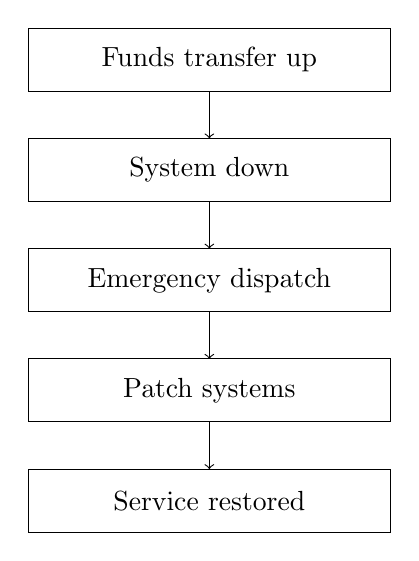
\begin{tikzpicture}[x=1cm,y=1cm]
\draw (-2.3,0.0) rectangle (2.3,0.8);
\node at (0,0.4) {Funds transfer up};

\draw (-2.3,-1.4) rectangle (2.3,-0.6);
\node at (0,-1.0) {System down};

\draw (-2.3,-2.8) rectangle (2.3,-2.0);
\node at (0,-2.4) {Emergency dispatch};

\draw (-2.3,-4.2) rectangle (2.3,-3.4);
\node at (0,-3.8) {Patch systems};

\draw (-2.3,-5.6) rectangle (2.3,-4.8);
\node at (0,-5.2) {Service restored};

\draw[->] (0,0.0) -- (0,-0.6);
\draw[->] (0,-1.4) -- (0,-2.0);
\draw[->] (0,-2.8) -- (0,-3.4);
\draw[->] (0,-4.2) -- (0,-4.8);
\end{tikzpicture}
\end{figure}

This little diagram should be read as a narrative spine rather than a systems-engineering drawing. Its purpose is to preserve the order of the lecture: first failure, then travel, then repair, then restoration.

\subsection{Question \& Answer}

\paragraph{Question.} What do we do when responsibility arrives before confidence?

\paragraph{Answer.} In this lecture, we do not wait for confidence to become psychologically complete. We enter the restoration chain and act on the system that is failing. The answer is procedural before it is emotional: bring the system back up, and let credibility be the consequence of performance under pressure.

That is why the lecture does not end with a motivational slogan at the beginning. It waits. The self-assessment is delayed until after the work has been done.

\section{People, Money, and Scrutiny}

At the end of the story, the speaker recaps the moment by naming three burdens at once: the amount of people, the amount of money, and the amount of scrutiny. This is a useful place to introduce one more compact object.

\begin{definition}
We define the pressure tuple
\begin{equation}
\boldsymbol{\pi}=(N,M,S),
\end{equation}
where \(N\) is the scale of people involved, \(M\) is the money at risk, and \(S\) is the level of scrutiny surrounding the event.
\end{definition}

We should not turn \(\boldsymbol{\pi}\) into a false precision. The speaker does not offer numbers, and we do not need them. What matters is that all three coordinates are large at once:

\begin{equation}
N \uparrow, \qquad M \uparrow, \qquad S \uparrow.
\end{equation}

The business lesson is then easier to state. A crisis becomes formative not merely because the system is broken, but because the system is broken while money is leaving, many people are implicated, and the event is highly visible. The conjunction matters.

There is also a quiet entrepreneurial principle here. Authority in real operations is often granted backward. It is recognized after the decisive act, not before it. The speaker's final line --- that this was where he figured out he could actually do this --- is the subjective form of that objective sequence.

\section{From Performance to Credibility}

We can summarize the movement of the lecture in one chain. First, youth makes the assignment feel unstable. Second, institutional failure raises the stakes. Third, time turns failure into accumulating loss. Fourth, intervention interrupts that accumulation. Fifth, restored service changes the speaker's estimate of himself.

One may express that final transition schematically as an update in self-belief:
\begin{equation}
C_{\text{after}} > C_{\text{before}},
\end{equation}
where \(C\) denotes operational self-confidence. This is not a measured variable from the transcript; it is a compact way of preserving the lecture's payoff. Confidence here is not treated as temperament. It is treated as the residue of action under conditions of consequence.

\section{Summary}

The chapter begins with a question about the biggest challenge in a career and answers it with an outage. The speaker was young, the client was large, the funds transfer system was down, and losses were mounting over a short interval. A simple linear downtime model,
\[
L(\Delta t)=r\,\Delta t,
\]
is enough to make the urgency legible without pretending to know more than the transcript gives us.

The core lesson is equally simple. Responsibility may arrive before confidence, but execution need not wait for inner certainty. In this case, restoration came first; the belief that one could do the job came after.